% =====================================================================
%  Fiche d'explication – Essai 9 : procédés de démarrage et de freinage
%  Aide personnelle (pas à rendre) – version française
%  Compilation : pdflatex erklaerung_fr.tex (2x)
% =====================================================================
\documentclass[11pt,a4paper]{article}
\usepackage[utf8]{inputenc}
\usepackage[T1]{fontenc}
\usepackage[french]{babel}
\usepackage{lmodern}
\usepackage{microtype}
\usepackage[a4paper,left=2.3cm,right=2.3cm,top=2.5cm,bottom=2.5cm]{geometry}
\usepackage{amsmath,amssymb}
\usepackage[locale=FR,per-mode=symbol]{siunitx}
\usepackage{graphicx}
\usepackage{booktabs}
\usepackage{float}
\usepackage{enumitem}
\setlist{itemsep=2pt,topsep=4pt}
\usepackage{xcolor}
\usepackage[colorlinks=true,linkcolor=black,urlcolor=blue!50!black]{hyperref}
\usepackage[most]{tcolorbox}
\usepackage{fancyhdr}

\graphicspath{{../bericht/abbildungen/}}
% automatisch erzeugt von auswertung/auswertung.py
\newcommand{\WJStahl}{0{,}3711}
\newcommand{\WJAlu}{0{,}1277}
\newcommand{\WJVorb}{0{,}3745}
\newcommand{\WdtBsp}{42{,}6}
\newcommand{\WtHDA}{1{,}20}
\newcommand{\WtHDB}{1{,}29}
\newcommand{\WtHDC}{1{,}40}
\newcommand{\WtHYA}{3{,}62}
\newcommand{\WtHYB}{3{,}92}
\newcommand{\WtHYC}{4{,}24}
\newcommand{\WdirektIeins}{50{,}66}
\newcommand{\WdirektUnull}{405}
\newcommand{\WdirektUeins}{388}
\newcommand{\WdirektPeins}{17896}
\newcommand{\WdirektQeins}{56162}
\newcommand{\Wdirektnend}{1499}
\newcommand{\WdirektIend}{4{,}58}
\newcommand{\WdirektPend}{1747}
\newcommand{\WdirektQend}{5175}
\newcommand{\Wdirekttneunacht}{1{,}14}
\newcommand{\Wdirektteinsvierfuenfnull}{1{,}10}
\newcommand{\WdirektE}{14509}
\newcommand{\WdirektdU}{4{,}3}
\newcommand{\WdirektIfak}{11{,}0}
\newcommand{\WdirektIN}{7{,}6}
\newcommand{\WfruehIeins}{15{,}51}
\newcommand{\WfruehUnull}{405}
\newcommand{\WfruehUeins}{400}
\newcommand{\WfruehPeins}{6685}
\newcommand{\WfruehQeins}{17788}
\newcommand{\Wfruehnend}{1497}
\newcommand{\WfruehIend}{4{,}59}
\newcommand{\WfruehPend}{1760}
\newcommand{\WfruehQend}{5173}
\newcommand{\Wfruehtneunacht}{2{,}65}
\newcommand{\Wfruehteinsvierfuenfnull}{2{,}62}
\newcommand{\WfruehE}{15389}
\newcommand{\WfruehdU}{1{,}2}
\newcommand{\WfruehIfak}{3{,}4}
\newcommand{\WfruehIN}{2{,}3}
\newcommand{\Wfruehtum}{1{,}91}
\newcommand{\Wfruehnum}{724}
\newcommand{\Wfruehpause}{0{,}16}
\newcommand{\WfruehIzwei}{45{,}91}
\newcommand{\WfruehUzwei}{384}
\newcommand{\WfruehPzwei}{20422}
\newcommand{\WfruehdUzwei}{5{,}1}
\newcommand{\WrichtigIeins}{15{,}51}
\newcommand{\WrichtigUnull}{405}
\newcommand{\WrichtigUeins}{400}
\newcommand{\WrichtigPeins}{5635}
\newcommand{\WrichtigQeins}{17779}
\newcommand{\Wrichtignend}{1497}
\newcommand{\WrichtigIend}{4{,}57}
\newcommand{\WrichtigPend}{1755}
\newcommand{\WrichtigQend}{5162}
\newcommand{\Wrichtigtneunacht}{3{,}86}
\newcommand{\Wrichtigteinsvierfuenfnull}{3{,}82}
\newcommand{\WrichtigE}{15754}
\newcommand{\WrichtigdU}{1{,}3}
\newcommand{\WrichtigIfak}{3{,}4}
\newcommand{\WrichtigIN}{2{,}3}
\newcommand{\Wrichtigtum}{3{,}60}
\newcommand{\Wrichtignum}{1443}
\newcommand{\Wrichtigpause}{0{,}14}
\newcommand{\WrichtigIzwei}{42{,}25}
\newcommand{\WrichtigUzwei}{402}
\newcommand{\WrichtigPzwei}{11284}
\newcommand{\WrichtigdUzwei}{0{,}9}
\newcommand{\WfalschIeins}{15{,}71}
\newcommand{\WfalschUnull}{405}
\newcommand{\WfalschUeins}{400}
\newcommand{\WfalschPeins}{5622}
\newcommand{\WfalschQeins}{18202}
\newcommand{\Wfalschnend}{1498}
\newcommand{\WfalschIend}{4{,}58}
\newcommand{\WfalschPend}{1781}
\newcommand{\WfalschQend}{5172}
\newcommand{\Wfalschtneunacht}{3{,}90}
\newcommand{\Wfalschteinsvierfuenfnull}{3{,}59}
\newcommand{\WfalschE}{15842}
\newcommand{\WfalschdU}{1{,}3}
\newcommand{\WfalschIfak}{3{,}4}
\newcommand{\WfalschIN}{2{,}4}
\newcommand{\Wfalschtum}{3{,}62}
\newcommand{\Wfalschnum}{1453}
\newcommand{\Wfalschpause}{0{,}15}
\newcommand{\WfalschIzwei}{50{,}91}
\newcommand{\WfalschUzwei}{401}
\newcommand{\WfalschPzwei}{19180}
\newcommand{\WfalschdUzwei}{1{,}0}
\newcommand{\WtHYum}{3{,}87}
\newcommand{\WdirektMBmittel}{52{,}7}
\newcommand{\WfruehMBmittel}{14{,}8}
\newcommand{\WrichtigMBmittel}{15{,}8}
\newcommand{\WfalschMBmittel}{15{,}9}
\newcommand{\WMkennDmittel}{48{,}8}
\newcommand{\WMkennYmittel}{16{,}1}
\newcommand{\WEkin}{2268}
\newcommand{\Wfedernnull}{1801}
\newcommand{\WfedertB}{0{,}88}
\newcommand{\Wfederts}{0{,}12}
\newcommand{\WfederMmit}{31{,}7}
\newcommand{\WfederMmax}{32{,}0}
\newcommand{\WfederUzkmax}{583}
\newcommand{\WfederErb}{0}
\newcommand{\Wfederverz}{2047}
\newcommand{\Wfedernullnnull}{1801}
\newcommand{\WfedernulltB}{0{,}90}
\newcommand{\Wfedernullts}{0{,}12}
\newcommand{\WfedernullMmit}{30{,}8}
\newcommand{\WfedernullMmax}{31{,}3}
\newcommand{\WfedernullUzkmax}{583}
\newcommand{\WfedernullErb}{0}
\newcommand{\Wfedernullverz}{1996}
\newcommand{\WdclnI}{1773}
\newcommand{\WdclIdcB}{14{,}1}
\newcommand{\WdclIeffB}{9{,}4}
\newcommand{\WdcltI}{1{,}03}
\newcommand{\WdcltnachI}{5{,}17}
\newcommand{\Wdclnnull}{1801}
\newcommand{\WdcltB}{6{,}20}
\newcommand{\Wdclts}{0{,}40}
\newcommand{\WdclMmit}{4{,}6}
\newcommand{\WdclMmax}{21{,}4}
\newcommand{\WdclUzkmax}{595}
\newcommand{\WdclErb}{0}
\newcommand{\Wdclverz}{290}
\newcommand{\WdcmnI}{1774}
\newcommand{\WdcmIdcB}{20{,}5}
\newcommand{\WdcmIeffB}{13{,}7}
\newcommand{\WdcmtI}{1{,}02}
\newcommand{\WdcmtnachI}{2{,}43}
\newcommand{\Wdcmnnull}{1801}
\newcommand{\WdcmtB}{3{,}45}
\newcommand{\Wdcmts}{0{,}41}
\newcommand{\WdcmMmit}{9{,}7}
\newcommand{\WdcmMmax}{33{,}9}
\newcommand{\WdcmUzkmax}{596}
\newcommand{\WdcmErb}{0}
\newcommand{\Wdcmverz}{521}
\newcommand{\WdcsnI}{1774}
\newcommand{\WdcsIdcB}{32{,}8}
\newcommand{\WdcsIeffB}{21{,}9}
\newcommand{\WdcstI}{1{,}03}
\newcommand{\WdcstnachI}{0{,}95}
\newcommand{\Wdcsnnull}{1801}
\newcommand{\WdcstB}{1{,}98}
\newcommand{\Wdcsts}{0{,}42}
\newcommand{\WdcsMmit}{25{,}5}
\newcommand{\WdcsMmax}{57{,}5}
\newcommand{\WdcsUzkmax}{596}
\newcommand{\WdcsErb}{0}
\newcommand{\Wdcsverz}{929}
\newcommand{\Wgenohnennull}{1801}
\newcommand{\WgenohnetB}{8{,}49}
\newcommand{\Wgenohnets}{0{,}09}
\newcommand{\WgenohneMmit}{2{,}9}
\newcommand{\WgenohneMmax}{19{,}6}
\newcommand{\WgenohneUzkmax}{815}
\newcommand{\WgenohneErb}{0}
\newcommand{\Wgenohneverz}{211}
\newcommand{\Wgenlnnull}{1801}
\newcommand{\WgenltB}{10{,}12}
\newcommand{\Wgenlts}{0{,}14}
\newcommand{\WgenlMmit}{2{,}4}
\newcommand{\WgenlMmax}{2{,}8}
\newcommand{\WgenlUzkmax}{724}
\newcommand{\WgenlErb}{512}
\newcommand{\Wgenlverz}{177}
\newcommand{\Wgenmnnull}{1801}
\newcommand{\WgenmtB}{5{,}13}
\newcommand{\Wgenmts}{0{,}10}
\newcommand{\WgenmMmit}{4{,}8}
\newcommand{\WgenmMmax}{5{,}8}
\newcommand{\WgenmUzkmax}{724}
\newcommand{\WgenmErb}{1365}
\newcommand{\Wgenmverz}{349}
\newcommand{\Wgensnnull}{1801}
\newcommand{\WgenstB}{0{,}87}
\newcommand{\Wgensts}{0{,}06}
\newcommand{\WgensMmit}{29{,}6}
\newcommand{\WgensMmax}{39{,}2}
\newcommand{\WgensUzkmax}{723}
\newcommand{\WgensErb}{1821}
\newcommand{\Wgensverz}{2061}
\newcommand{\WRb}{28}
\newcommand{\WPRbmax}{7760}
\newcommand{\WgensErbAnteil}{80}


\newtcolorbox{merke}{colback=green!5,colframe=green!45!black,fonttitle=\bfseries,
  title={À retenir},boxrule=0.6pt,arc=1mm}
\newtcolorbox{einfach}{colback=yellow!7,colframe=orange!70!black,fonttitle=\bfseries,
  title={Expliqué simplement},boxrule=0.6pt,arc=1mm}
\newtcolorbox{frage}[1]{colback=blue!4,colframe=blue!50!black,fonttitle=\bfseries\small,
  title={#1},boxrule=0.6pt,arc=1mm}
\newtcolorbox{achtung}{colback=red!4,colframe=red!60!black,fonttitle=\bfseries,
  title={Attention / à vérifier toi-même},boxrule=0.6pt,arc=1mm}
\newcommand{\de}[1]{\textit{(all.\ « #1 »)}}

\pagestyle{fancy}\fancyhf{}
\fancyhead[L]{Fiche d'explication V9}\fancyhead[R]{Démarrage et freinage}
\fancyfoot[C]{\thepage}

\begin{document}
\sloppy
\begin{center}
{\LARGE\bfseries Fiche d'explication -- Essai 9}\\[4pt]
{\Large Procédés de démarrage et de freinage de la machine asynchrone}\\[2pt]
{\normalsize\itshape (Versuch 9: Anlauf- und Bremsverfahren)}\\[6pt]
{\normalsize Tous les points de l'essai expliqués pas à pas -- pour comprendre, apprendre et préparer l'oral (Testat)}
\end{center}

\begin{achtung}
Le rapport et les diagrammes sont en allemand, comme au laboratoire. Les termes allemands
importants sont donc indiqués entre parenthèses. Le lexique à la fin de ce document (section~\ref{sec:lexique}) traduit les termes des diagrammes.
\end{achtung}

\tableofcontents
\newpage

% =====================================================================
\section{De quoi parle l'essai ? (Le fil rouge)}
% =====================================================================
L'essai comporte deux parties :
\begin{enumerate}
\item \textbf{Démarrage} \de{Anlauf} : comment mettre en marche un moteur asynchrone sans trop
  charger le réseau ? On compare le \emph{démarrage direct en triangle}
  \de{direkter Dreieckanlauf} et le \emph{démarrage étoile-triangle}
  \de{Stern-Dreieck-Anlauf}. Avant l'essai, on calcule la durée du démarrage.
\item \textbf{Freinage} \de{Bremsen} : comment arrêter rapidement un moteur avec volant d'inertie ?
  On compare le \emph{frein à ressort} \de{Federkraftbremse}, le \emph{freinage par courant
  continu} \de{DC-Bremse} et le \emph{freinage en génératrice} \de{generatorisches Bremsen},
  avec et sans résistance de freinage \de{Bremswiderstand}.
\end{enumerate}
La formule unique qui relie tout est l'\textbf{équation du mouvement} \de{Bewegungsgleichung} :
\[
  J\cdot\frac{\mathrm d\omega}{\mathrm dt} = M_\mathrm{moteur} - M_\mathrm{charge}.
\]
\begin{einfach}
Un couple accélère ou freine une masse en rotation, comme une force accélère ou freine
une voiture ($F = m\cdot a$). Ici, $M = J\cdot\alpha$ :
\begin{itemize}
\item $J$ est la « masse en rotation » (moment d'inertie, en \si{kg.m^2}),
\item $\alpha = \mathrm d\omega/\mathrm dt$ est l'accélération angulaire.
\end{itemize}
Cette formule permet de calculer \emph{dans les deux sens} :
\begin{itemize}
\item couple connu $\Rightarrow$ calcul du temps (préparation, temps de démarrage) ;
\item vitesse mesurée $\Rightarrow$ calcul du couple (exploitation des mesures).
\end{itemize}
\end{einfach}

% =====================================================================
\section{Les bases à comprendre}
% =====================================================================
\subsection{Pourquoi le courant de démarrage est-il si grand ?}
À l'arrêt, un moteur asynchrone est comme un \textbf{transformateur dont le secondaire est en
court-circuit} : la cage du rotor est un anneau en court-circuit. À l'arrêt (glissement
$s=1$), le champ du stator passe à pleine vitesse devant le rotor. Une grande tension est
induite et un grand courant circule. Il n'est limité que par la petite impédance de court-circuit.

\textbf{Glissement} \de{Schlupf} : $s = \dfrac{n_s - n}{n_s}$, avec $n_s = \dfrac{f}{p}$
(vitesse synchrone). À \SI{50}{Hz} et $p=2$ : $n_s = \SI{1500}{tr/min}$.
\begin{itemize}
\item À l'arrêt : $s=1$, courant élevé.
\item À la vitesse nominale \SI{1420}{tr/min} : $s\approx0{,}05$, courant faible.
\end{itemize}
\textbf{Mesuré :} démarrage direct \SI{\WdirektIeins}{A}, soit \WdirektIN{} fois le courant
nominal de \SI{6,65}{A}. C'est exactement la plage habituelle (5 à 8 fois).

\subsection{Pourquoi la tension du réseau chute-t-elle ?}
Le réseau (transformateur et câbles) a une impédance interne $Z_k = R_k + \mathrm jX_k$.
Quand un grand courant circule, une partie de la tension y chute, et le moteur reçoit moins de tension.

\textbf{Pourquoi la chute est-elle si forte au démarrage ?}
\begin{itemize}
\item Le courant de démarrage est presque purement réactif (mesuré : $\cos\varphi\approx0{,}3$).
\item Pour un transformateur, $X_k$ est beaucoup plus grand que $R_k$.
\item La chute de tension $\mathrm jX_k\cdot I$ est donc presque parallèle à la tension du
      réseau et la réduit directement.
\end{itemize}
C'est le \textbf{triangle de Kapp} \de{Kapp'sches Dreieck} :
$\Delta U \approx I\,(R_k\cos\varphi + X_k\sin\varphi)$.
Avec $\sin\varphi\approx1$, c'est presque toute la valeur $X_k\cdot I$ qui agit.

\subsection{Étoile et triangle -- les facteurs \texorpdfstring{$\sqrt3$}{racine de 3} et 3}
\begin{center}
\begin{tabular}{@{}lcc@{}}
\toprule
& Étoile (Y) & Triangle ($\Delta$)\\
\midrule
Tension sur un enroulement & $400/\sqrt3 = \SI{230}{V}$ & \SI{400}{V}\\
Courant d'enroulement & $\frac{1}{\sqrt3}\cdot I_{\mathrm{enr},\Delta}$ & $I_{\mathrm{enr},\Delta}$\\
Courant de ligne (réseau) & $\frac13\cdot I_{\mathrm{ligne},\Delta}$ & $I_{\mathrm{ligne},\Delta} = \sqrt3\,I_{\mathrm{enr},\Delta}$\\
Couple ($\sim U^2$) & $\frac13\cdot M_\Delta$ & $M_\Delta$\\
\bottomrule
\end{tabular}
\end{center}
\textbf{D'où vient le facteur 3 pour le courant de ligne ?}
\begin{itemize}
\item En étoile, la tension d'enroulement est $\sqrt3$ fois plus petite, le courant d'enroulement aussi.
\item En triangle, le courant de ligne est en plus $\sqrt3$ fois plus grand que le courant d'enroulement.
\item Ensemble : $\sqrt3\cdot\sqrt3 = 3$.
\end{itemize}
\textbf{Mesuré :} $\WdirektIeins/\WrichtigIeins\approx3{,}3$, cela correspond bien.

\textbf{Pourquoi $M\sim U^2$ ?} Le flux est proportionnel à $U$, le courant rotorique aussi.
Le couple vaut flux fois courant, donc il est proportionnel à $U^2$.

\begin{merke}
L'étoile-triangle réduit le courant \emph{et} le couple à un tiers. Cela ne fonctionne que si la
charge au démarrage est faible (ventilateurs, pompes, volant sans charge). Pour des convoyeurs
ou des engins de levage en charge, un tiers du couple ne suffit souvent pas.
\end{merke}

\subsection{La caractéristique de couple \texorpdfstring{$M(n)$}{M(n)}}
Points importants (voir fig.~\ref{fig:kenn}) :
\begin{itemize}
\item \textbf{Couple de démarrage} \de{Anzugsmoment} à $n=0$ : ici \SI{46}{Nm}.
\item \textbf{Couple de selle} \de{Sattelmoment} : petit creux vers \SI{200}{tr/min}. Il est dû aux
      harmoniques, typique des rotors à cage.
\item \textbf{Couple de décrochage} \de{Kippmoment}, le maximum : env.\ \SI{56}{Nm} vers \SI{1000}{tr/min}.
\item Ensuite, le couple chute fortement et devient nul à $n_s = \SI{1500}{tr/min}$.
      Sans glissement, rien n'est induit, donc il n'y a pas de couple.
\end{itemize}
\begin{figure}[H]\centering
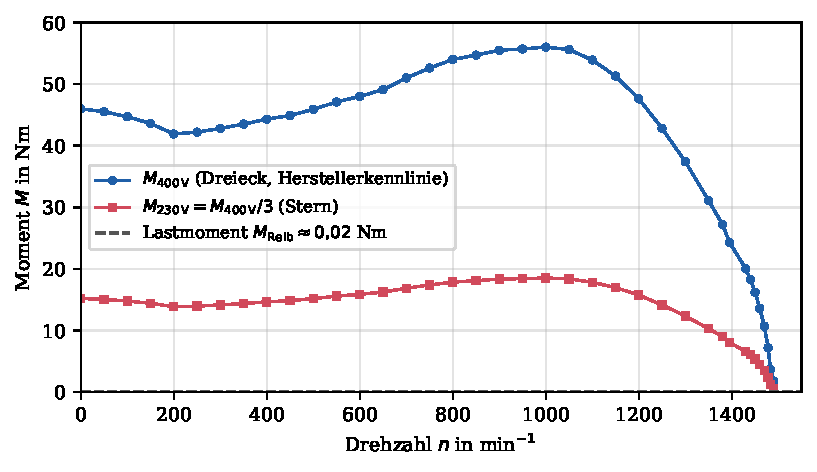
\includegraphics[width=0.8\textwidth]{v_kennlinie}
\caption{Caractéristique de couple (relevée dans la notice) et caractéristique en étoile (un tiers)}
\label{fig:kenn}
\end{figure}

\subsection{Le moment d'inertie \texorpdfstring{$J$}{J}}
Pour un disque plein : $J = \frac12 m r^2$, avec le rayon $r = d/2 = \SI{0,15}{m}$.
\begin{itemize}
\item Disque en acier (démarrage) : $J = 0{,}5\cdot32{,}99\cdot0{,}15^2 = \SI{\WJStahl}{kg.m^2}$.
\item Disque en aluminium (freinage) : $J = 0{,}5\cdot11{,}35\cdot0{,}15^2 = \SI{\WJAlu}{kg.m^2}$.
\item La notice indique \SI{0,3745}{kg.m^2}. C'est un peu plus que le disque en acier seul ;
      le moment d'inertie du rotor du moteur est probablement inclus.
\end{itemize}

% =====================================================================
\section{Préparation : calcul du temps de démarrage, pas à pas}
% =====================================================================
\textbf{Idée :} on découpe la plage de vitesse en petits morceaux (par ex.\ \SI{50}{tr/min}).
Dans chaque morceau, on considère le couple comme constant et on calcule la durée du morceau.
À la fin, on additionne toutes les durées. C'est l'\textbf{intégration numérique}.

\textbf{Démonstration de la formule :}
\begin{align*}
J\,\frac{\Delta\omega}{\Delta t} &= M
\quad\Rightarrow\quad \Delta t = \frac{J\,\Delta\omega}{M},
\qquad \Delta\omega = 2\pi\,\Delta n\;(\Delta n \text{ en } \si{\per\second})\\
\Rightarrow\quad \Delta t &= \frac{2\pi\,J\,\Delta n}{M}.
\end{align*}

\textbf{Exemple} pour le premier pas, de 0 à \SI{50}{tr/min}, en triangle :
\begin{enumerate}
\item Convertir le pas de vitesse en \si{\per\second} : $\Delta n = 50/60 = \SI{0,833}{\per\second}$.
\item Remplacer : $\Delta t = 2\pi\cdot0{,}3745\cdot0{,}833/46 = \SI{0,0426}{s}\approx\SI{42}{ms}$.
      C'est exactement la valeur de la notice.
\item En étoile, le couple n'est que $46/3 = \SI{15,3}{Nm}$ : le pas dure trois fois plus
      longtemps, env.\ \SI{128}{ms}.
\end{enumerate}

\textbf{Méthode dans Excel} (ou comme dans le script Python) :
\begin{enumerate}
\item Colonne A : vitesse $n$ ; colonne B : couple $M_{400}$ (relevé).
\item Colonne C : $M_{230} = B/3$.
\item Colonne D : couple moyen de l'intervalle $(B_i+B_{i+1})/2$, moins \SI{0,02}{Nm} de frottement.
\item Colonne E : $\Delta t = 2\pi\cdot J\cdot(A_{i+1}-A_i)/60/D$.
\item Colonne F : temps cumulé $t$.
\item Tracer $n$ en fonction de $t$ -- \textbf{non normalisé}, donc avec de vraies secondes et
      des tr/min, comme demandé dans la notice.
\end{enumerate}

\textbf{Résultat :}
\begin{itemize}
\item Triangle : \SI{\WtHDB}{s} jusqu'à \SI{1450}{tr/min}.
\item Étoile : \SI{\WtHYB}{s} jusqu'à \SI{1450}{tr/min}, exactement trois fois plus long.
\end{itemize}
Conclusion : en étoile, il faut commuter après environ \SIrange{3,6}{3,9}{s}.

\begin{achtung}
\begin{itemize}
\item Juste avant \SI{1500}{tr/min}, $M\to0$ et $\Delta t$ devient très grand. C'est pourquoi on
      ne calcule que jusqu'à \SI{1450}{} ou \SI{1480}{tr/min}. Tu dois pouvoir le justifier.
\item J'ai relevé la caractéristique sur la figure de la notice. Si vous avez le fichier CSV de
      StudIP avec la caractéristique, utilise ses valeurs. Les temps changeront un peu.
\end{itemize}
\end{achtung}

\begin{figure}[H]\centering
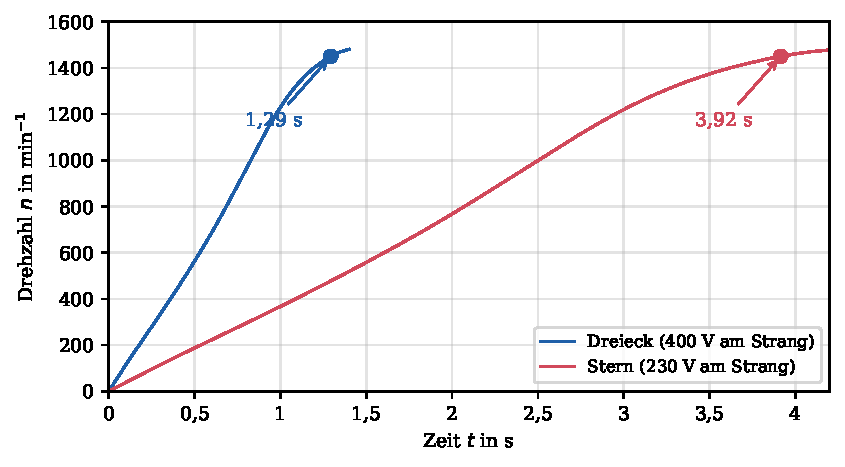
\includegraphics[width=0.8\textwidth]{v_hochlauf}
\caption{Démarrage calculé (Dreieck = triangle, Stern = étoile)}
\end{figure}

% =====================================================================
\section{Essais de démarrage : que montrent les diagrammes ?}
% =====================================================================
\textbf{Comment lire :} chaque diagramme de démarrage comporte quatre parties superposées :
\begin{enumerate}
\item vitesse $n$,
\item courant $I$,
\item tension $U$,
\item puissance active $P$ et puissance réactive $Q$.
\end{enumerate}
La zone grise est la pause de commutation, pendant laquelle le moteur est brièvement sans courant.

\subsection{Démarrage direct en triangle (fichier \texttt{Stern-Dreieck\_direkt.csv})}
\begin{figure}[H]\centering
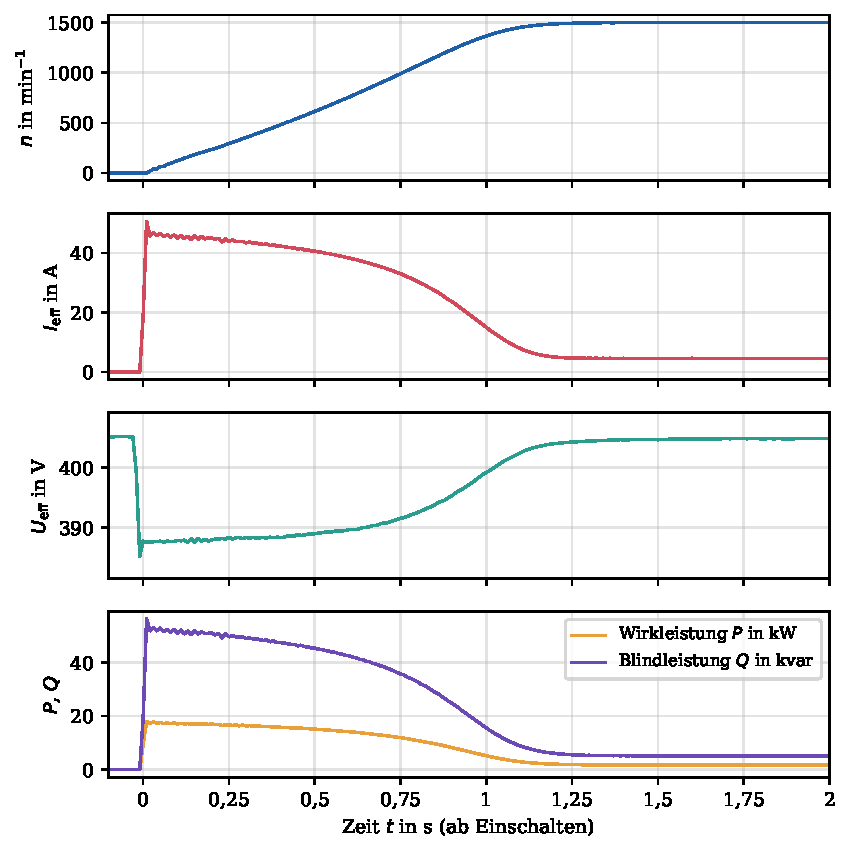
\includegraphics[width=0.72\textwidth]{a_direkt}
\end{figure}
\textbf{Déroulement :}
\begin{enumerate}
\item Mise sous tension : le courant monte à env.\ \SI{50}{A}, la tension baisse de \SI{405}{V}
      à \SI{388}{V} (\SI{\WdirektdU}{\percent}).
\item Le courant reste élevé longtemps : jusqu'au glissement de décrochage, l'impédance est faible.
\item À partir d'env.\ \SI{1000}{tr/min} (couple de décrochage), le courant tombe rapidement au
      courant à vide de \SI{4,6}{A} et la tension remonte.
\item Après \SI{\Wdirekttneunacht}{s}, le démarrage est terminé.
\end{enumerate}
\textbf{Puissances :}
\begin{itemize}
\item $Q\approx3\cdot P$, donc $\cos\varphi\approx0{,}3$ : le courant de démarrage est surtout réactif.
\item À vide, $P\approx\SI{1,75}{kW}$ : ce sont les pertes fer, mécaniques et cuivre à vide.
      Le moteur n'a pas de charge.
\end{itemize}

\subsection{Étoile-triangle commuté trop tôt}
\begin{figure}[H]\centering
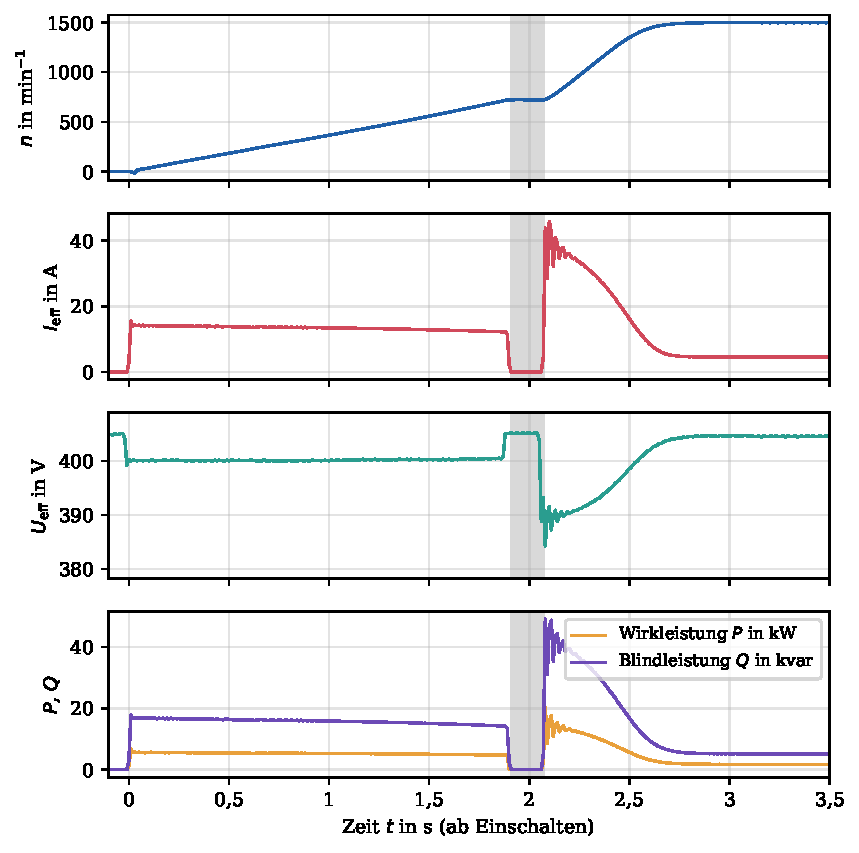
\includegraphics[width=0.72\textwidth]{a_frueh}
\end{figure}
\textbf{Déroulement :}
\begin{enumerate}
\item En étoile, le courant n'est que d'env.\ \SI{15}{A}, un tiers. La tension chute à peine.
\item La machine accélère trois fois plus lentement.
\item La commutation a lieu déjà à \SI{\Wfruehnum}{tr/min}, encore loin de la vitesse nominale :
      le glissement est encore grand.
\item En triangle, presque tout le courant de démarrage revient donc : \SI{\WfruehIzwei}{A}.
      La tension descend même à \SI{\WfruehUzwei}{V}.
\end{enumerate}
\textbf{Conclusion :} le réseau subit quand même un fort pic de courant. L'étoile-triangle n'a
presque rien apporté.
\begin{achtung}
Selon la notice, le temps de commutation devait être de \SI{0,5}{s}. Dans les mesures, la
commutation n'a lieu qu'après env.\ \SI{1,9}{s}. Une autre valeur a peut-être été réglée le jour
de l'essai. Vérifie dans tes notes. Le rapport utilise la valeur mesurée dans les données.
\end{achtung}

\subsection{Étoile-triangle commuté au bon moment}
\begin{figure}[H]\centering
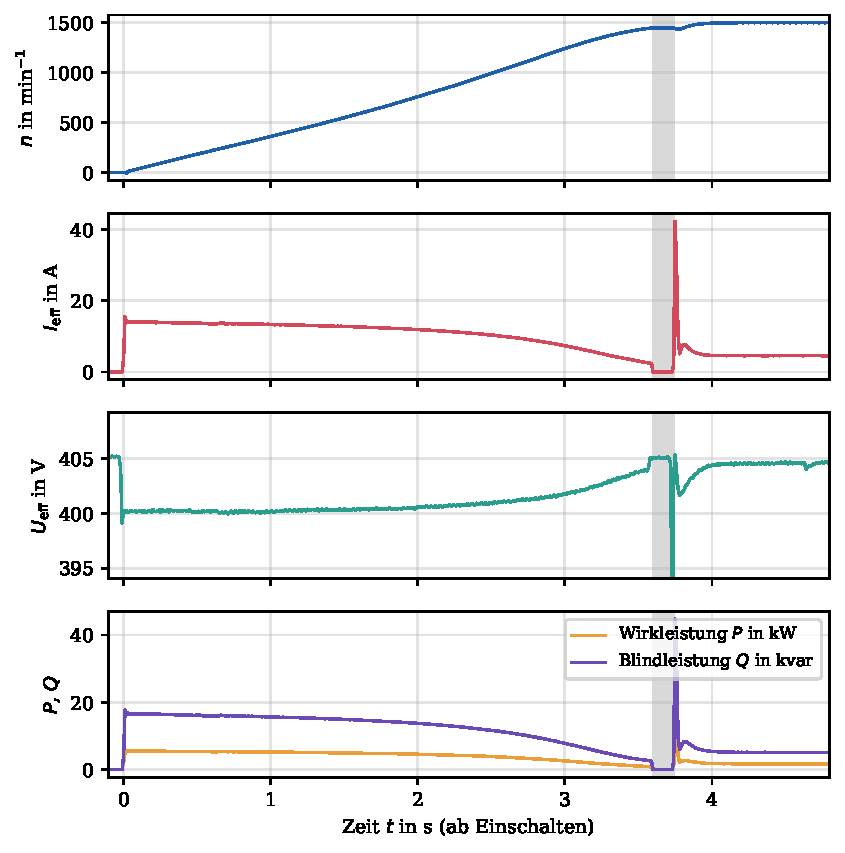
\includegraphics[width=0.72\textwidth]{a_richtig}
\end{figure}
\textbf{Déroulement :}
\begin{enumerate}
\item Commutation à \SI{\Wrichtignum}{tr/min}, après \SI{\Wrichtigtum}{s}. Cela correspond au calcul.
\item Le courant était déjà descendu à env.\ \SI{2,5}{A}.
\item À la commutation, il n'y a qu'un pic très court (env.\ \SI{20}{ms}).
\end{enumerate}
\textbf{D'où vient ce pic ?} Pendant la courte pause, le rotor est encore magnétisé et produit
sa propre tension, la \emph{tension rémanente} \de{Restspannung}. Au moment de la reconnexion,
la tension du réseau et la tension rémanente ne coïncident pas exactement. Un court courant
d'équilibrage apparaît.

\subsection{Étoile-triangle mal câblé}
\begin{figure}[H]\centering
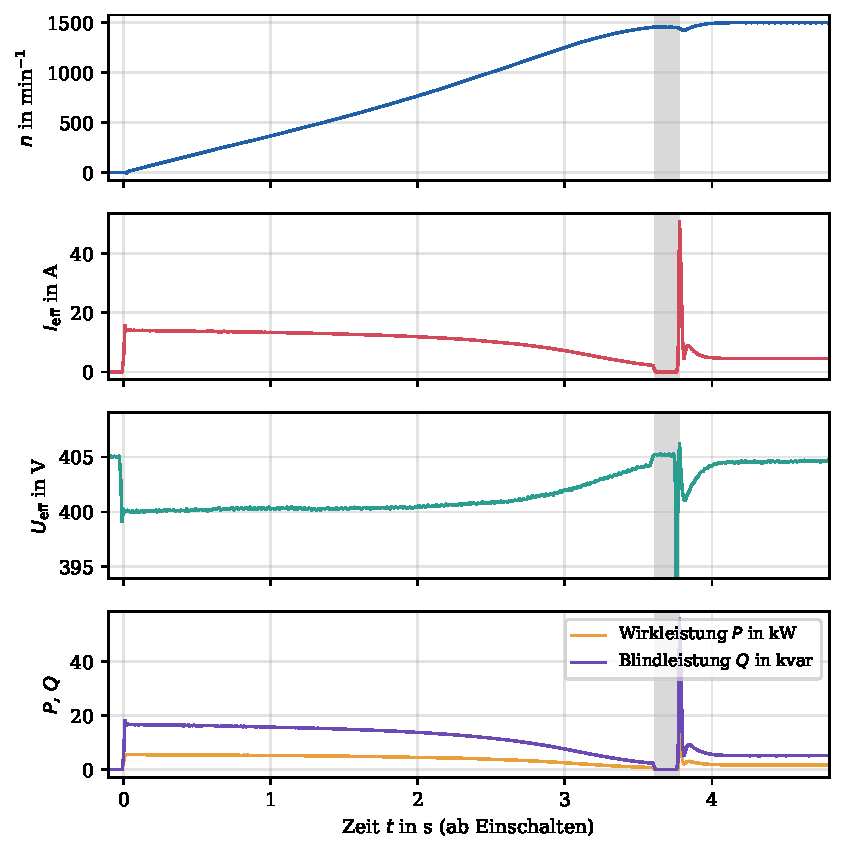
\includegraphics[width=0.72\textwidth]{a_falsch}
\end{figure}
\textbf{Différence avec le bon câblage :} même vitesse de commutation, mais
\begin{itemize}
\item le pic de courant est plus grand (\SI{\WfalschIzwei}{A} au lieu de \SI{\WrichtigIzwei}{A}),
\item le pic de puissance active est presque deux fois plus élevé,
\item la vitesse chute brièvement d'env.\ \SI{30}{tr/min}.
\end{itemize}
\begin{einfach}
\begin{itemize}
\item En passant d'étoile à triangle, la tension de chaque enroulement tourne de \SI{30}{\degree}.
\item Le sens de ce saut (en avant ou en arrière) dépend du raccordement des extrémités
      d'enroulement U2, V2, W2 à L1, L2, L3.
\item Avec le bon câblage, la nouvelle tension du réseau est proche de la tension rémanente
      du rotor : le pic est petit.
\item Avec un mauvais câblage, l'angle entre les deux est plus grand. Le courant d'équilibrage
      est plus grand et freine même un instant le moteur (d'où la chute de vitesse).
\end{itemize}
\end{einfach}
\begin{achtung}
C'est l'explication habituelle. Ce qui était exactement mal câblé le jour de l'essai, seules
tes notes ou l'encadrant peuvent le dire. Demande en cas de doute.
\end{achtung}

\subsection{Couple d'accélération calculé à partir des mesures}
\textbf{Méthode :}
\begin{enumerate}
\item Dériver la vitesse par rapport au temps : $\mathrm dn/\mathrm dt$.
\item Multiplier par $J$ et $2\pi$ : $M_B = J\cdot2\pi\cdot\mathrm dn/\mathrm dt$.
\end{enumerate}
Comme la vitesse mesurée est bruitée (sauts de $\pm\SI{1}{tr/min}$), il faut d'abord la lisser.
J'ai utilisé un \emph{filtre de Savitzky-Golay}, qui ajuste une parabole par morceaux sur les points.

\textbf{Variante Excel :} quotient de différences $(n_{i+5}-n_{i-5})/(t_{i+5}-t_{i-5})$ sur
plusieurs points. Cela lisse aussi.
\begin{figure}[H]\centering
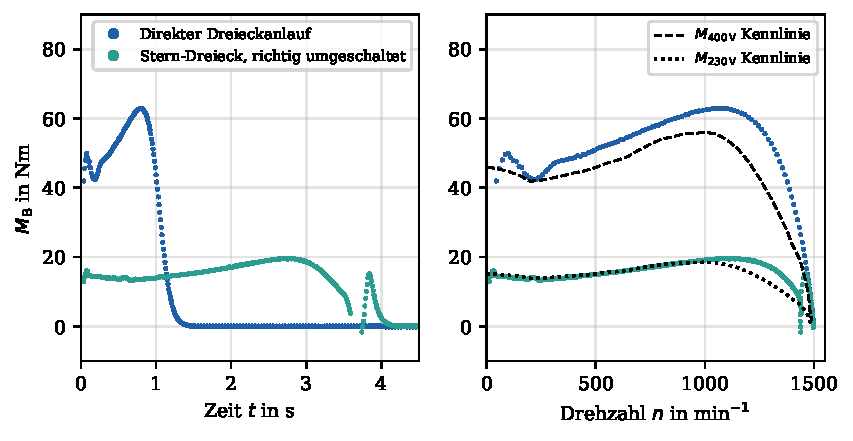
\includegraphics[width=0.9\textwidth]{a_moment}
\end{figure}
\textbf{Résultat :}
\begin{itemize}
\item La forme de la caractéristique se retrouve dans la mesure : selle, décrochage, chute.
\item En étoile, mesure et calcul coïncident presque exactement.
\item En triangle, le couple mesuré est env.\ \SI{8}{\percent} plus grand que la caractéristique.
      C'est pourquoi le temps de démarrage mesuré est plus court que le calcul
      (\SI{\Wdirektteinsvierfuenfnull}{s} au lieu de \SI{\WtHDB}{s}).
\end{itemize}

\begin{merke}
Raisons de l'écart entre mesure et calcul :
\begin{itemize}
\item La caractéristique du fabricant a des tolérances.
\item La tension était de \SI{405}{V} au lieu de \SI{400}{V}. Avec $M\sim U^2$, cela donne
      $+\SI{2,5}{\percent}$ de couple.
\item La caractéristique a été relevée sur une figure.
\item La valeur de $J$ de la notice est un peu plus grande.
\item La fin exacte du démarrage est difficile à définir.
\end{itemize}
\end{merke}

\subsection{Énergie -- une observation intéressante en plus}
\begin{itemize}
\item À la fin, le volant contient $E = \frac12J\omega^2\approx\SI{4,6}{kJ}$.
\item Pourtant, env.\ \SIrange{14,5}{15,8}{kJ} ont été pris au réseau.
\item \textbf{Raison :} lors du démarrage à vide d'une machine asynchrone, le rotor dissipe en
      chaleur autant d'énergie que celle stockée dans le volant. S'y ajoutent les pertes stator et fer.
\item L'étoile-triangle n'économise donc \emph{pas d'énergie}. Il répartit seulement le courant
      sur une durée plus longue et évite les pics élevés.
\end{itemize}

% =====================================================================
\section{Essais de freinage : que montrent les diagrammes ?}
% =====================================================================
\textbf{Situation de départ :}
\begin{itemize}
\item Moteur sur variateur de fréquence \de{Frequenzumrichter, FU}, vitesse env.\
      \SI{1800}{tr/min} (\SI{60}{Hz}), disque en aluminium.
\item $t=0$ est l'ordre de freinage.
\item Énergie dans le disque : $E_\mathrm{cin} = \frac12\cdot0{,}1277\cdot(2\pi\cdot30)^2\approx\SI{2270}{J}$.
\item Couple de freinage : $M_\mathrm{Br} = -J\cdot2\pi\cdot\mathrm dn/\mathrm dt$.
\end{itemize}

\subsection{Le variateur en 4 blocs}
\begin{enumerate}
\item \textbf{Redresseur} \de{Gleichrichter} (diodes) : transforme la tension alternative du réseau
  en tension continue. Il peut seulement \emph{prendre} de l'énergie, \emph{pas la renvoyer au réseau}.
\item \textbf{Circuit intermédiaire} \de{Zwischenkreis} (condensateur) :
  env.\ $\sqrt2\cdot\SI{400}{V}\approx\SI{565}{V}$, mesuré \SI{580}{V}.
\item \textbf{Hacheur de freinage} \de{Brems-Chopper} avec résistance de freinage : un transistor
  qui connecte la résistance quand la tension du circuit intermédiaire est trop élevée.
\item \textbf{Onduleur} \de{Wechselrichter} (IGBT) : produit un courant triphasé de fréquence quelconque.
\end{enumerate}
\begin{merke}
Le plus important pour toutes les questions de freinage : le redresseur à diodes est un sens
unique. L'énergie de freinage ne peut pas retourner au réseau. Elle doit être transformée en
chaleur : dans le moteur (frein CC), dans la résistance de freinage ou dans le frein à friction.
\end{merke}

\subsection{Vue d'ensemble}
\begin{figure}[H]\centering
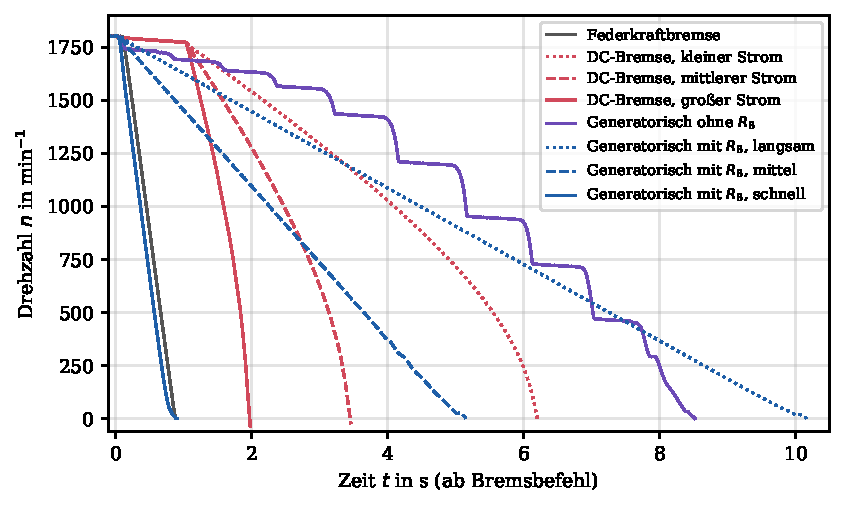
\includegraphics[width=0.85\textwidth]{b_vergleich_n}
\end{figure}

\subsection{Frein à ressort}
\textbf{Fonctionnement :}
\begin{itemize}
\item Un ressort presse les garnitures de frein ensemble.
\item Un électroaimant maintient le frein ouvert (« desserré », \de{gelüftet}).
\item Plus de courant $\Rightarrow$ l'aimant relâche $\Rightarrow$ le ressort freine.
\end{itemize}
\textbf{Mesure :}
\begin{itemize}
\item env.\ \SI{\Wfederts}{s} de retard (temps de retombée : le champ magnétique doit d'abord disparaître),
\item ensuite la vitesse diminue \textbf{linéairement}, donc le couple est constant : env.\ \SI{\WfederMmit}{Nm},
\item arrêt après \SI{\WfedertB}{s}.
\end{itemize}
\textbf{Pourquoi le couple est-il constant ?} Le frottement sec (Coulomb) ne dépend pas de la
vitesse : force de frottement $=\mu\cdot$ force du ressort.

\subsection{Freinage par courant continu (frein CC)}
\textbf{Fonctionnement :}
\begin{itemize}
\item Le variateur envoie un courant continu dans l'enroulement du stator. Il se crée un champ
      magnétique \emph{fixe}.
\item Le rotor qui tourne coupe ce champ. Un courant est induit et un couple de freinage
      apparaît, comme dans un frein à courants de Foucault.
\end{itemize}
\textbf{Mesure :}
\begin{itemize}
\item D'abord rien pendant env.\ \SI{1}{s} : le variateur attend que la tension rémanente du moteur
      disparaisse (temps de démagnétisation). Sinon, il y aurait un courant de court-circuit.
\item Ensuite, freinage avec \SI{\WdclIdcB}{A}, \SI{\WdcmIdcB}{A} ou \SI{\WdcsIdcB}{A}.
\item Le temps de freinage passe de \SI{\WdcltnachI}{s} à \SI{\WdcmtnachI}{s} puis à \SI{\WdcstnachI}{s}.
\end{itemize}
\begin{figure}[H]\centering
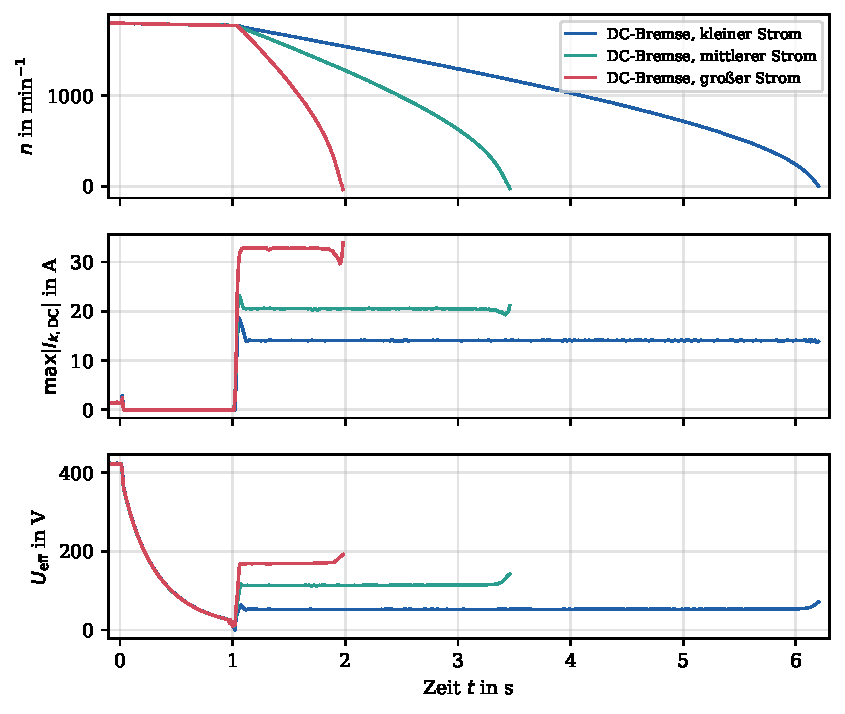
\includegraphics[width=0.72\textwidth]{b_dc}
\end{figure}
\textbf{Trois choses que tu dois savoir expliquer :}
\begin{enumerate}
\item \textbf{Couple $\sim I^2$ :} le champ est $\sim I$, le courant rotorique induit aussi
  $\sim I$, donc le couple est $\sim I^2$. Mesuré : courant $\times1{,}45\Rightarrow$ couple
  $\times2{,}1$ ; courant $\times2{,}33\Rightarrow$ couple $\times5{,}5$. Ça correspond !
\item \textbf{Le couple augmente vers la fin} (la courbe devient plus raide) : à vitesse élevée,
  la fréquence rotorique est élevée. Le rotor est alors fortement inductif et le courant est
  « mal placé » par rapport au champ. À faible vitesse, c'est mieux. Le maximum est donc juste
  avant l'arrêt, comme la caractéristique du moteur, mais inversée.
\item \textbf{Pas de couple de maintien :} à $n=0$, rien n'est induit, donc pas de couple.
  Une charge suspendue (grue) descendrait lentement. De plus, toute l'énergie est dissipée
  \emph{dans le moteur}, qui chauffe.
\end{enumerate}

\subsection{Freinage en génératrice sans résistance de freinage}
\textbf{Fonctionnement :} le variateur baisse la fréquence. La machine tourne alors plus vite
que le champ ($s<0$) et devient génératrice. L'énergie va dans le circuit intermédiaire.

\textbf{Mesure et explication :}
\begin{itemize}
\item $U_\mathrm{ZK}$ monte de \SI{580}{V} jusqu'à \SI{\WgenohneUzkmax}{V}.
\item En cas de surtension, le variateur bloque les impulsions. Le courant est alors nul et le
      moteur tourne en roue libre.
\item Quand $U_\mathrm{ZK}$ est redescendue, une courte impulsion de freinage suit, et le cycle recommence.
\item Résultat : la vitesse baisse par paliers, arrêt seulement après \SI{\WgenohnetB}{s}.
\end{itemize}
\begin{figure}[H]\centering
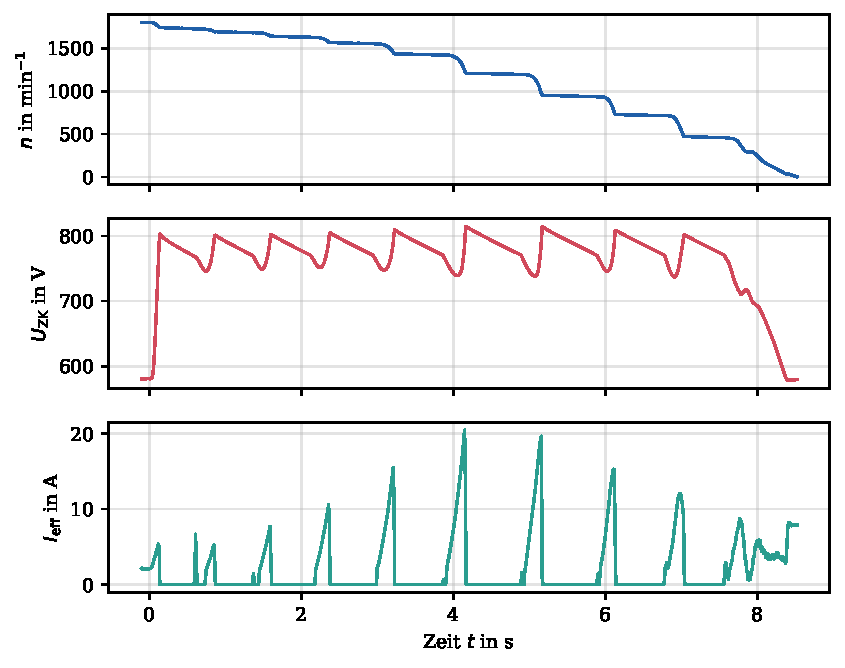
\includegraphics[width=0.72\textwidth]{b_gen0}
\end{figure}

\subsection{Freinage en génératrice avec résistance de freinage}
\textbf{Mesure :}
\begin{itemize}
\item Le hacheur limite $U_\mathrm{ZK}$ à env.\ \SI{720}{V}.
\item Le moteur suit exactement la rampe : la vitesse diminue linéairement, le couple est constant.
\item Temps de freinage : lent \SI{\WgenltB}{s}, moyen \SI{\WgenmtB}{s}, rapide \SI{\WgenstB}{s}.
\item Rapide : la résistance absorbe jusqu'à \SI{7,8}{kW}. Au total env.\ \SI{\WgensErb}{J} y
      sont dissipés, soit \SI{\WgensErbAnteil}{\percent} de l'énergie cinétique. Le reste, ce sont
      les pertes dans le moteur et le variateur.
\item Avec la rampe lente, le hacheur ne commute presque pas : les pertes du moteur et du
      variateur suffisent presque pour la faible puissance de freinage.
\end{itemize}
\textbf{Estimation de la résistance de freinage :} le hacheur commute le courant par impulsions.
\begin{itemize}
\item Rapport cyclique : $D = (I_\mathrm{moy}/I_\mathrm{eff})^2$.
\item Courant à l'état passant : $I_\mathrm{on} = I_\mathrm{moy}/D$.
\item Résistance : $R = U_\mathrm{ZK}/I_\mathrm{on}\approx\SI{\WRb}{\ohm}$.
\end{itemize}
\begin{figure}[H]\centering
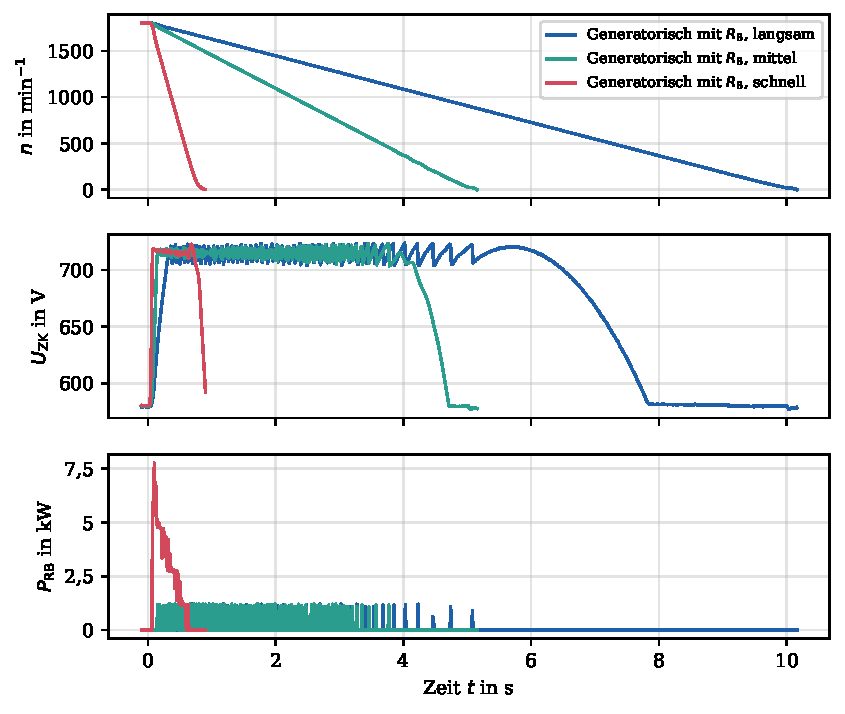
\includegraphics[width=0.72\textwidth]{b_gen}
\end{figure}

\subsection{Comparaison des couples de freinage}
\begin{figure}[H]\centering
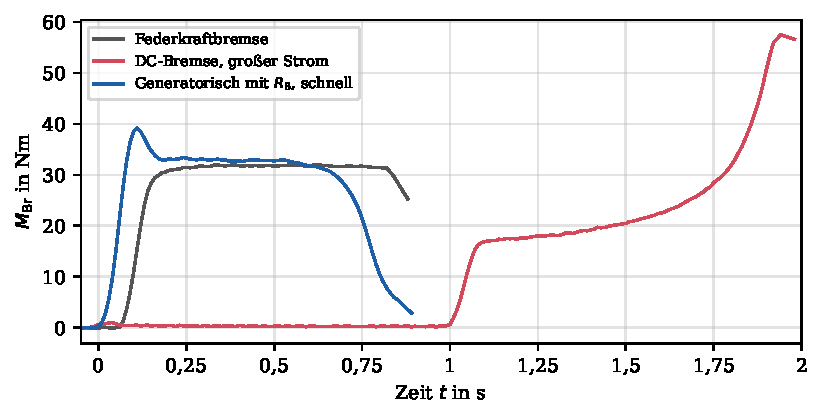
\includegraphics[width=0.8\textwidth]{b_moment_zoom}
\end{figure}
\begin{center}
\begin{tabular}{@{}lccc@{}}
\toprule
Procédé & Allure du couple & Maintien ? & Où l'énergie est-elle dissipée ?\\
\midrule
Frein à ressort & constant & oui & garnitures de frein\\
Frein CC & augmente vers l'arrêt & non & moteur (rotor)\\
Génératrice sans $R_B$ & seulement des impulsions & non & pertes, condensateur\\
Génératrice avec $R_B$ & constant (rampe) & non & résistance de freinage\\
\bottomrule
\end{tabular}
\end{center}

% =====================================================================
\section{Les questions de la notice -- réponses avec tes propres mots}
% =====================================================================
\begin{frage}{D'où vient la chute de tension et comment la réduire ?}
\textbf{Cause :}
\begin{itemize}
\item Le grand courant de démarrage traverse l'impédance interne du réseau (transformateur et câbles).
\item Il est presque purement réactif, et le transformateur est surtout inductif.
\item La chute de tension réduit donc directement la tension du réseau.
\end{itemize}
\textbf{Remèdes :}
\begin{itemize}
\item Étoile-triangle (bien réglé), démarreur progressif, variateur de fréquence,
      autotransformateur de démarrage.
\item Transformateur plus puissant avec un petit $u_k$, câbles plus gros ou plus courts.
\end{itemize}
\end{frage}

\begin{frage}{Comparaison entre temps de démarrage calculé et mesuré}
\begin{itemize}
\item Triangle : calculé \SI{\WtHDB}{s}, mesuré \SI{\Wdirektteinsvierfuenfnull}{s}.
\item Étoile : calculé env.\ \SI{\WtHYum}{s}, mesuré \SI{\Wrichtigtum}{s} (jusqu'à \SI{1443}{tr/min}).
\end{itemize}
La mesure est un peu plus rapide, car la machine réelle a plus de couple (tolérance, \SI{405}{V},
erreur de lecture). L'allure correspond très bien.
\end{frage}

\begin{frage}{Calculer le couple d'accélération et le comparer avec la préparation}
\begin{itemize}
\item Formule : $M = J\cdot2\pi\cdot\mathrm dn/\mathrm dt$ avec $J = \SI{0,3711}{kg.m^2}$.
\item Résultat : la forme ressemble à la caractéristique. Moyenne en triangle
      \SI{\WdirektMBmittel}{Nm} (caractéristique \SI{\WMkennDmittel}{Nm}), en étoile
      \SI{\WrichtigMBmittel}{Nm} (caractéristique \SI{\WMkennYmittel}{Nm}).
\end{itemize}
\end{frage}

\begin{frage}{Pourquoi le freinage en génératrice sans résistance est-il beaucoup plus lent ?}
\begin{itemize}
\item L'énergie ne peut pas retourner au réseau, car le redresseur à diodes est à sens unique.
\item Sans résistance, l'énergie n'a nulle part où aller.
\item $U_\mathrm{ZK}$ monte jusqu'à la limite de surtension et le variateur interrompt le freinage.
\item Avec résistance, l'énergie est dissipée en chaleur et la rampe est respectée :
      \SI{0,87}{s} au lieu de \SI{8,5}{s}.
\end{itemize}
\end{frage}

\begin{frage}{Quel procédé convient comme arrêt d'urgence ?}
Le \textbf{frein à ressort}, parce qu'il
\begin{itemize}
\item freine \emph{sans courant} (sécurité positive, principe du courant de repos),
\item agit même en cas de coupure de réseau ou de défaut du variateur,
\item \emph{maintient} la charge à l'arrêt.
\end{itemize}
Tous les procédés électriques ont besoin du réseau et du variateur. En pratique, on combine :
d'abord un freinage en génératrice (ménage les garnitures), puis le frein à ressort se ferme
(catégorie d'arrêt 1).
\end{frage}

% =====================================================================
\section{Questions possibles pour l'oral (Testat)}
% =====================================================================
\begin{enumerate}[label=\textbf{Q\arabic*:},leftmargin=2.2em]
\item \emph{Pourquoi le courant de démarrage vaut-il 5 à 8 fois le courant nominal ?}\\
  À $s=1$, le moteur est comme un transformateur en court-circuit : seule la petite impédance
  de court-circuit limite le courant.
\item \emph{Pourquoi le courant ne baisse-t-il fortement qu'après le couple de décrochage ?}\\
  Ce n'est qu'à faible glissement que la résistance rotorique $R_2'/s$ devient grande. Avant,
  l'impédance reste faible.
\item \emph{De quel facteur le courant et le couple baissent-ils en étoile ?}\\
  Tous deux à un tiers. Raison : tension d'enroulement $/\sqrt3$, $M\sim U^2$, courant de
  ligne $\sqrt3\cdot\sqrt3 = 3$.
\item \emph{Quand ne doit-on pas utiliser l'étoile-triangle ?}\\
  Quand le couple de charge au démarrage dépasse un tiers du couple moteur, par ex.\ convoyeurs
  lourds ou engins de levage. Il vaut mieux utiliser un variateur.
\item \emph{Que se passe-t-il si on commute trop tôt ?}\\
  Un deuxième pic de courant, presque comme au démarrage direct.
\item \emph{Que se passe-t-il si le moteur ne monte pas en vitesse en étoile ?}\\
  Il reste bloqué à la vitesse où $M_{230} = M_\mathrm{charge}$. Il absorbe longtemps un
  courant élevé et surchauffe.
\item \emph{Comment calcule-t-on le couple à partir de la vitesse ?}\\
  $M = J\cdot2\pi\cdot\mathrm dn/\mathrm dt$, avec $n$ en \si{\per\second}.
\item \emph{Quel est le $J$ d'un disque plein ?}\\
  $\frac12 m r^2$. Attention : le rayon, pas le diamètre !
\item \emph{Pourquoi le frein CC n'a-t-il pas de couple de maintien ?}\\
  Sans mouvement, rien n'est induit.
\item \emph{Où va l'énergie lors du freinage CC ?}\\
  Dans le moteur (rotor et stator), qui chauffe.
\item \emph{Pourquoi $U_\mathrm{ZK}$ monte-t-elle lors du freinage en génératrice ?}\\
  L'énergie va dans le condensateur, et le redresseur à diodes ne peut pas la renvoyer au réseau.
\item \emph{Qu'est-ce qu'un hacheur de freinage ?}\\
  Un transistor qui connecte la résistance de freinage au circuit intermédiaire à partir d'un
  seuil de tension.
\item \emph{Comment pourrait-on utiliser l'énergie de freinage au lieu de la dissiper ?}\\
  Avec un variateur réversible (Active Front End) ou un circuit intermédiaire commun à plusieurs entraînements.
\item \emph{Pourquoi le frein à ressort est-il à sécurité positive ?}\\
  C'est le ressort qui freine ; le courant ne fait que \emph{desserrer}. Si le courant disparaît,
  le frein agit.
\item \emph{Pourquoi le frein CC a-t-il besoin d'un temps d'attente avant l'injection ?}\\
  Le moteur est encore magnétisé et produit une tension rémanente. Si le variateur injectait
  tout de suite, il y aurait des surintensités.
\end{enumerate}

% =====================================================================
\section{Formulaire}
% =====================================================================
\begin{center}
\renewcommand{\arraystretch}{1.5}
\begin{tabular}{@{}ll@{}}
\toprule
Vitesse synchrone & $n_s = f/p$\\
Glissement & $s = (n_s-n)/n_s$\\
Puissance -- couple & $P = M\cdot\omega = M\cdot2\pi n$\\
Couple et tension & $M\sim U^2$, \quad $M_{230} = \frac13M_{400}$\\
Équation du mouvement & $J\,\mathrm d\omega/\mathrm dt = M_\mathrm{mot} - M_\mathrm{charge}$\\
Pas de temps & $\Delta t = 2\pi J\Delta n/M$\\
Moment d'inertie (disque plein) & $J = \frac12 m r^2$\\
Énergie cinétique & $E = \frac12 J\omega^2$\\
Chute de tension (Kapp) & $\Delta U\approx I(R_k\cos\varphi + X_k\sin\varphi)$\\
Facteur de puissance & $\cos\varphi = P/\sqrt{P^2+Q^2}$\\
Couple de freinage CC & $M_\mathrm{Br}\sim I_\mathrm{DC}^2$\\
\bottomrule
\end{tabular}
\end{center}

% =====================================================================
\section{Lexique allemand -- français (termes des diagrammes)}
\label{sec:lexique}
% =====================================================================
\begin{center}
\small
\begin{tabular}{@{}p{0.47\textwidth}p{0.47\textwidth}@{}}
\toprule
Allemand & Français\\
\midrule
Drehzahl $n$ & vitesse de rotation\\
Zeit $t$ (ab Einschalten / ab Bremsbefehl) & temps (depuis la mise en marche / l'ordre de freinage)\\
Moment, Drehmoment $M$ & couple\\
Wirkleistung / Blindleistung & puissance active / réactive\\
Strom / Spannung & courant / tension\\
Stern / Dreieck & étoile / triangle\\
Anlauf / Hochlauf & démarrage / montée en vitesse\\
umschalten, Umschaltpause & commuter, pause de commutation\\
zu früh / richtig / falsch verdrahtet & trop tôt / correct / mal câblé\\
Kennlinie, Rechnung & caractéristique, calcul\\
Zwischenkreisspannung $U_\mathrm{ZK}$ & tension du circuit intermédiaire\\
Bremswiderstand $R_B$ & résistance de freinage\\
Federkraftbremse & frein à ressort\\
DC-Bremse, kleiner/mittlerer/großer Strom & frein CC, courant faible/moyen/fort\\
Generatorisch, langsam/mittel/schnell & en génératrice, lent/moyen/rapide\\
Kippmoment / Sattelmoment / Anzugsmoment & couple de décrochage / de selle / de démarrage\\
Schlupf & glissement\\
Frequenzumrichter (FU) & variateur de fréquence\\
Schwungmasse / Schwungscheibe & volant d'inertie\\
\bottomrule
\end{tabular}
\end{center}

% =====================================================================
\section{Remarques importantes sur tes fichiers}
% =====================================================================
\begin{itemize}
\item \textbf{Non utilisés :} les fichiers \texttt{F\_Kennline\_Dreick.csv},
  \texttt{F\_Kennline\_Stern.csv} et \texttt{Messung\_f87Hz\_*.csv} n'appartiennent pas à V9.
  Ce sont des caractéristiques en fréquence ou un fonctionnement à 87 Hz, probablement d'un
  autre essai. Ils ne sont donc pas dans le rapport.
\item \textbf{Noms des fichiers :} \texttt{Stern-Dreieck\_direkt.csv} est le
  \emph{démarrage direct en triangle} (on le voit au courant de démarrage de \SI{50}{A}).
\item \textbf{À compléter avant de rendre :} page de garde (noms, numéros de matricule, groupe,
  date). Vérifie aussi le temps de commutation « trop tôt » (\SI{0,5}{s} selon la notice,
  \SI{1,9}{s} dans les données).
\item \textbf{Modifier :} pour changer des valeurs, modifie les données ou le script
  \texttt{auswertung/auswertung.py}, exécute-le (\texttt{python3 auswertung.py}) et recompile
  le rapport. Toutes les valeurs du texte se mettent à jour automatiquement.
\end{itemize}
\end{document}
